% Created by tikzDevice version 0.10.1 on 2017-05-08 20:28:59
% !TEX encoding = UTF-8 Unicode


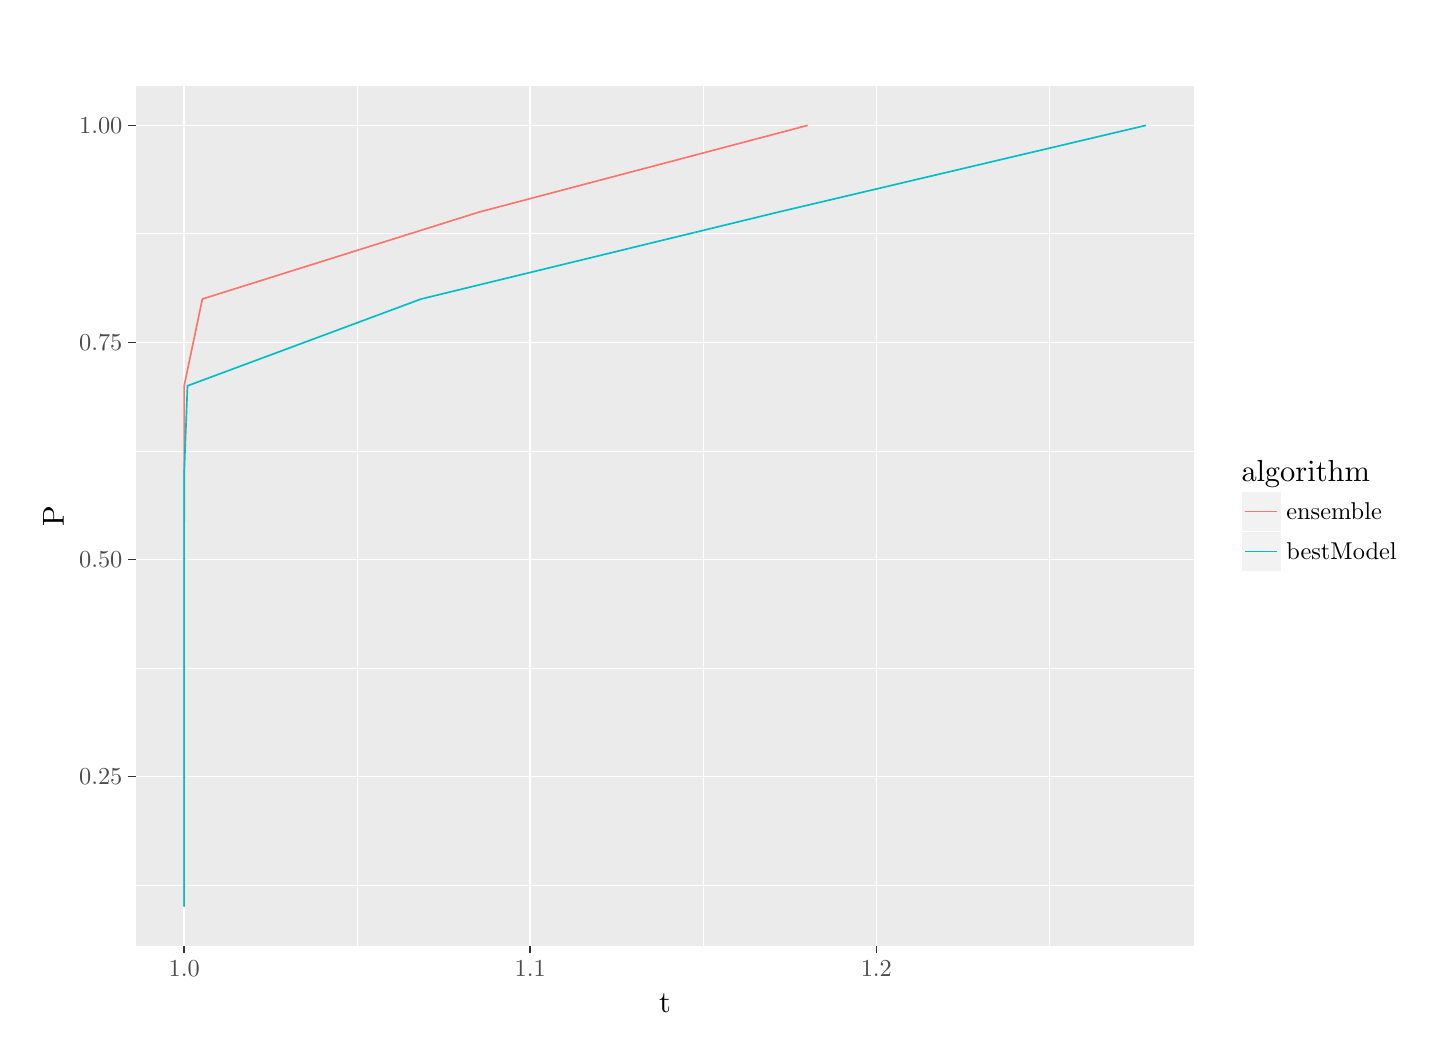
\begin{tikzpicture}[x=1pt,y=1pt]
\definecolor{fillColor}{RGB}{255,255,255}
\path[use as bounding box,fill=fillColor,fill opacity=0.00] (0,0) rectangle (505.89,361.35);
\begin{scope}
\path[clip] (  0.00,  0.00) rectangle (505.89,361.35);
\definecolor{drawColor}{RGB}{255,255,255}
\definecolor{fillColor}{RGB}{255,255,255}

\path[draw=drawColor,line width= 0.6pt,line join=round,line cap=round,fill=fillColor] (  0.00, -0.00) rectangle (505.89,361.35);
\end{scope}
\begin{scope}
\path[clip] ( 39.17, 29.59) rectangle (421.48,340.16);
\definecolor{fillColor}{gray}{0.92}

\path[fill=fillColor] ( 39.17, 29.59) rectangle (421.48,340.16);
\definecolor{drawColor}{RGB}{255,255,255}

\path[draw=drawColor,line width= 0.3pt,line join=round] ( 39.17, 51.55) --
	(421.48, 51.55);

\path[draw=drawColor,line width= 0.3pt,line join=round] ( 39.17,129.97) --
	(421.48,129.97);

\path[draw=drawColor,line width= 0.3pt,line join=round] ( 39.17,208.40) --
	(421.48,208.40);

\path[draw=drawColor,line width= 0.3pt,line join=round] ( 39.17,286.83) --
	(421.48,286.83);

\path[draw=drawColor,line width= 0.3pt,line join=round] (119.08, 29.59) --
	(119.08,340.16);

\path[draw=drawColor,line width= 0.3pt,line join=round] (244.14, 29.59) --
	(244.14,340.16);

\path[draw=drawColor,line width= 0.3pt,line join=round] (369.20, 29.59) --
	(369.20,340.16);

\path[draw=drawColor,line width= 0.6pt,line join=round] ( 39.17, 90.76) --
	(421.48, 90.76);

\path[draw=drawColor,line width= 0.6pt,line join=round] ( 39.17,169.19) --
	(421.48,169.19);

\path[draw=drawColor,line width= 0.6pt,line join=round] ( 39.17,247.61) --
	(421.48,247.61);

\path[draw=drawColor,line width= 0.6pt,line join=round] ( 39.17,326.04) --
	(421.48,326.04);

\path[draw=drawColor,line width= 0.6pt,line join=round] ( 56.54, 29.59) --
	( 56.54,340.16);

\path[draw=drawColor,line width= 0.6pt,line join=round] (181.61, 29.59) --
	(181.61,340.16);

\path[draw=drawColor,line width= 0.6pt,line join=round] (306.67, 29.59) --
	(306.67,340.16);
\definecolor{drawColor}{RGB}{248,118,109}

\path[draw=drawColor,line width= 0.6pt,line join=round] ( 56.54, 43.70) --
	( 56.54, 75.07) --
	( 56.54,106.45) --
	( 56.54,137.82) --
	( 56.54,169.19) --
	( 56.54,200.56) --
	( 56.54,231.93) --
	( 63.12,263.30) --
	(162.98,294.67) --
	(281.86,326.04);
\definecolor{drawColor}{RGB}{0,191,196}

\path[draw=drawColor,line width= 0.6pt,line join=round] ( 56.54, 43.70) --
	( 56.54, 75.07) --
	( 56.54,106.45) --
	( 56.54,137.82) --
	( 56.54,169.19) --
	( 56.56,200.56) --
	( 57.75,231.93) --
	(142.18,263.30) --
	(271.10,294.67) --
	(404.11,326.04);
\end{scope}
\begin{scope}
\path[clip] (  0.00,  0.00) rectangle (505.89,361.35);
\definecolor{drawColor}{gray}{0.30}

\node[text=drawColor,anchor=base east,inner sep=0pt, outer sep=0pt, scale=  0.88] at ( 34.22, 87.73) {0.25};

\node[text=drawColor,anchor=base east,inner sep=0pt, outer sep=0pt, scale=  0.88] at ( 34.22,166.16) {0.50};

\node[text=drawColor,anchor=base east,inner sep=0pt, outer sep=0pt, scale=  0.88] at ( 34.22,244.58) {0.75};

\node[text=drawColor,anchor=base east,inner sep=0pt, outer sep=0pt, scale=  0.88] at ( 34.22,323.01) {1.00};
\end{scope}
\begin{scope}
\path[clip] (  0.00,  0.00) rectangle (505.89,361.35);
\definecolor{drawColor}{gray}{0.20}

\path[draw=drawColor,line width= 0.6pt,line join=round] ( 36.42, 90.76) --
	( 39.17, 90.76);

\path[draw=drawColor,line width= 0.6pt,line join=round] ( 36.42,169.19) --
	( 39.17,169.19);

\path[draw=drawColor,line width= 0.6pt,line join=round] ( 36.42,247.61) --
	( 39.17,247.61);

\path[draw=drawColor,line width= 0.6pt,line join=round] ( 36.42,326.04) --
	( 39.17,326.04);
\end{scope}
\begin{scope}
\path[clip] (  0.00,  0.00) rectangle (505.89,361.35);
\definecolor{drawColor}{gray}{0.20}

\path[draw=drawColor,line width= 0.6pt,line join=round] ( 56.54, 26.84) --
	( 56.54, 29.59);

\path[draw=drawColor,line width= 0.6pt,line join=round] (181.61, 26.84) --
	(181.61, 29.59);

\path[draw=drawColor,line width= 0.6pt,line join=round] (306.67, 26.84) --
	(306.67, 29.59);
\end{scope}
\begin{scope}
\path[clip] (  0.00,  0.00) rectangle (505.89,361.35);
\definecolor{drawColor}{gray}{0.30}

\node[text=drawColor,anchor=base,inner sep=0pt, outer sep=0pt, scale=  0.88] at ( 56.54, 18.58) {1.0};

\node[text=drawColor,anchor=base,inner sep=0pt, outer sep=0pt, scale=  0.88] at (181.61, 18.58) {1.1};

\node[text=drawColor,anchor=base,inner sep=0pt, outer sep=0pt, scale=  0.88] at (306.67, 18.58) {1.2};
\end{scope}
\begin{scope}
\path[clip] (  0.00,  0.00) rectangle (505.89,361.35);
\definecolor{drawColor}{RGB}{0,0,0}

\node[text=drawColor,anchor=base,inner sep=0pt, outer sep=0pt, scale=  1.10] at (230.32,  5.50) {t};
\end{scope}
\begin{scope}
\path[clip] (  0.00,  0.00) rectangle (505.89,361.35);
\definecolor{drawColor}{RGB}{0,0,0}

\node[text=drawColor,rotate= 90.00,anchor=base,inner sep=0pt, outer sep=0pt, scale=  1.10] at ( 13.08,184.87) {P};
\end{scope}
\begin{scope}
\path[clip] (  0.00,  0.00) rectangle (505.89,361.35);
\definecolor{fillColor}{RGB}{255,255,255}

\path[fill=fillColor] (432.86,159.13) rectangle (500.39,210.61);
\end{scope}
\begin{scope}
\path[clip] (  0.00,  0.00) rectangle (505.89,361.35);
\definecolor{drawColor}{RGB}{0,0,0}

\node[text=drawColor,anchor=base west,inner sep=0pt, outer sep=0pt, scale=  1.10] at (438.55,197.35) {algorithm};
\end{scope}
\begin{scope}
\path[clip] (  0.00,  0.00) rectangle (505.89,361.35);
\definecolor{drawColor}{RGB}{255,255,255}
\definecolor{fillColor}{gray}{0.95}

\path[draw=drawColor,line width= 0.6pt,line join=round,line cap=round,fill=fillColor] (438.55,179.28) rectangle (453.01,193.73);
\end{scope}
\begin{scope}
\path[clip] (  0.00,  0.00) rectangle (505.89,361.35);
\definecolor{drawColor}{RGB}{248,118,109}

\path[draw=drawColor,line width= 0.6pt,line join=round] (440.00,186.51) -- (451.56,186.51);
\end{scope}
\begin{scope}
\path[clip] (  0.00,  0.00) rectangle (505.89,361.35);
\definecolor{drawColor}{RGB}{255,255,255}
\definecolor{fillColor}{gray}{0.95}

\path[draw=drawColor,line width= 0.6pt,line join=round,line cap=round,fill=fillColor] (438.55,164.82) rectangle (453.01,179.28);
\end{scope}
\begin{scope}
\path[clip] (  0.00,  0.00) rectangle (505.89,361.35);
\definecolor{drawColor}{RGB}{0,191,196}

\path[draw=drawColor,line width= 0.6pt,line join=round] (440.00,172.05) -- (451.56,172.05);
\end{scope}
\begin{scope}
\path[clip] (  0.00,  0.00) rectangle (505.89,361.35);
\definecolor{drawColor}{RGB}{0,0,0}

\node[text=drawColor,anchor=base west,inner sep=0pt, outer sep=0pt, scale=  0.88] at (454.82,183.47) {ensemble};
\end{scope}
\begin{scope}
\path[clip] (  0.00,  0.00) rectangle (505.89,361.35);
\definecolor{drawColor}{RGB}{0,0,0}

\node[text=drawColor,anchor=base west,inner sep=0pt, outer sep=0pt, scale=  0.88] at (454.82,169.02) {bestModel};
\end{scope}
\end{tikzpicture}

